\documentclass[../../main.tex]{subfiles}
\begin{document}

\begin{flushright}
\footnotesize\textit{【自動文字起こし・要確認】}
\end{flushright}

\noindent
\textbf{[解]} $V_1$ の表面上の点 $P(x,y,z)$ とする。この立体の $x+y = 2k \; (0 \le k \le 1)$ での切り断面は $H_k(k,k,0)$ を中心とし、半径 $\sqrt{2}(1-k)$ の円であるから、右下図のようである。この時、$x+y = t$ の点は $y$ 座標が $2k - t$ であり、$z$ 座標は、$k$ の正負で以下のようになる。

\medskip

\noindent
$1^\circ \; k \ge 0$
\[
(t-k)^2 + (2k-t-k)^2 + z^2 = 2(1-k)^2
\]
\[
z^2 = 2\{ (1-k)^2 - (t-k)^2 \} = 2(1-t) \{ -2k + (1+t) \}
\]

\noindent
$2^\circ \; k \le 0$
\[
(t-k)^2 + (2k-t-k)^2 + z^2 = 2(1+k)^2
\]
\[
z^2 = 2\{ (1+k)^2 - (t-k)^2 \} = 2(1+t) \{ 2k + (1-t) \}
\]

\noindent
次に $k$ を動かす。$-1 \le y \le 1$ から、
\[
\dfrac{t-1}{2} \le k \le \dfrac{t+1}{2}
\]
で考えれば良い。$y = 2k - t \implies k = \dfrac{y+t}{2}$ だから $0 \le k \le 1$ とあわせて、以下のようになる。

\medskip

\noindent
① $\dfrac{t-1}{2} \le k \le 0$\\
$\dfrac{t-1}{2} \le \dfrac{y+t}{2} \le 0 \implies -1 \le y \le -t$ の時、$2^\circ$ から
\[
z^2 = 2(1+t)(y+1) \quad \cdots \star_1
\]

\noindent
② $0 \le k \le \dfrac{t+1}{2}$\\
$0 \le \dfrac{y+t}{2} \le \dfrac{t+1}{2} \implies -t \le y \le 1$ の時、$1^\circ$ から
\[
z^2 = 2(1-t)(1-y) \quad \cdots \star_2
\]

\noindent
以上を図示すると右図斜線部のようになるから，この面積を$S(t)$とすると
\begin{align}
S(t) &= \left( \dfrac{1}{6 \cdot 2(1+t)} + \dfrac{1}{6 \cdot 2(1-t)} \right) \left( 2 \sqrt{2(1-t^2)} \right)^3 \quad (\star_1, \star_2 \text{より}) \\
&= \dfrac{1}{12} \left( \dfrac{1}{1+t} + \dfrac{1}{1-t} \right) \cdot 8 \cdot 2\sqrt{2} (1-t^2) \sqrt{1-t^2} \\
&= \dfrac{8}{3} \sqrt{2} \sqrt{1-t^2}
\end{align}
$t=1$ の時も $S(1) = 0$ となるのでこの式で良い。よって
\[
S(t) = \dfrac{8}{3} \sqrt{2} \sqrt{1-t^2} \hfill \text{固}
\]

\begin{center}
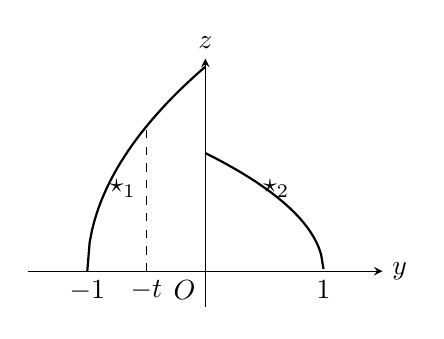
\begin{tikzpicture}[scale=1.5, >=stealth]
  \draw[->] (-1.5,0) -- (1.5,0) node[right] {$y$};
  \draw[->] (0,-0.3) -- (0,1.8) node[above] {$z$};
  \node[below left] at (0,0) {$O$};
  
  \draw[thick, domain=-1:0, samples=50] plot (\x, {sqrt(2*(1+0.5)*(\x+1))});
  \draw[thick, domain=0:1, samples=50] plot (\x, {sqrt(2*(1-0.5)*(1-\x))});
  
  \draw[dashed] (-1,0) node[below] {$-1$} -- (-1,0);
  \draw[dashed] (1,0) node[below] {$1$} -- (1,0);
  \draw[dashed] (-0.5,0) node[below] {$-t$} -- (-0.5, {sqrt(2*(1.5)*0.5)});
  
  \node at (-0.7, 0.7) {$\star_1$};
  \node at (0.6, 0.7) {$\star_2$};
\end{tikzpicture}
\end{center}

\bigskip

\noindent
\paragraph{(2)}

対称性から、求める体積 $V$, $V'$ のうち $0 \le x$ のものを $V'$ として、
\[
V = 2 V' \quad \cdots ③
\]
とできる。$V_2$ を $x=t$ で切った時の切断面は、$y$ と $z$ 軸に関して対称だから、共通部分は右図のようになる。この面積 $T(t)$ は
\begin{align}
T(t) &= 2 \cdot \dfrac{1}{6 \cdot 2(1-t)} \left( 2\sqrt{2(1-t)} \right)^3 \\
&= \dfrac{1}{6} \cdot 8 \sqrt{2} \sqrt{1-t} = \dfrac{8}{3} \sqrt{2} \sqrt{1-t}
\end{align}
だから、
\begin{align}
V' &= \int_0^1 T(t) dt \\
&= \dfrac{8}{3}\sqrt{2} \int_0^1 \sqrt{1-t} \, dt \\
&= \dfrac{8}{3}\sqrt{2} \left[ -\dfrac{2}{3} (1-t)^{\dfrac{3}{2}} \right]_0^1 = \dfrac{16}{9} \sqrt{2}
\end{align}
となり、③から
\[
V = \dfrac{32}{9}\sqrt{2} \hfill \text{固}
\]
である。

\end{document}
